\documentclass[11pt,a4paper]{article}
\usepackage[utf8]{inputenc}
\usepackage[margin=0.8in]{geometry}
\usepackage{amsmath,amssymb,amsthm}
\usepackage{tcolorbox}
\usepackage{tikz}
\usetikzlibrary{patterns,calc,arrows.meta,angles,quotes}
\usepackage{hyperref}
\usepackage{microtype}
\usepackage{lmodern}
\usepackage{xcolor}
\usepackage{fancyhdr}
\usepackage{booktabs}
\usepackage{enumitem}

\setlength{\headheight}{16pt}

\definecolor{primary}{HTML}{0D47A1}    % Deep Blue
\definecolor{secondary}{HTML}{1976D2}  % Medium Blue
\definecolor{accent}{HTML}{E3F2FD}     % Light Blue Accent
\definecolor{grayborder}{HTML}{CFD8DC} % Soft border gray
\definecolor{graybg}{HTML}{F8F9FA}     % Soft background gray
\definecolor{proofcolor}{HTML}{2E7D32} % Dark Green for proofs
\definecolor{examcolor}{HTML}{C62828}  % Dark Red for important questions

\hypersetup{
    colorlinks=true,
    linkcolor=primary,
    filecolor=magenta,      
    urlcolor=secondary,
    pdftitle={MTB 202 Statics and Dynamics Perfect Master Notes - BHU},
    pdfauthor={Aryan (sciqb.com)},
}

\pagestyle{fancy}
\fancyhf{}
\fancyhead[L]{\sffamily\bfseries\color{primary} MTB 202: Statics \& Dynamics -- Perfect Master Notes}
\fancyhead[R]{\sffamily\color{primary}\bfseries\href{https://sciqb.com}{sciqb.com}}
\fancyfoot[L]{\sffamily\color{gray}Notes by Aryan (BHU MTB 202)}
\fancyfoot[C]{\sffamily\color{gray}\thepage}
\fancyfoot[R]{\sffamily\color{secondary}\bfseries\href{https://sciqb.com}{sciqb.com}}
\renewcommand{\headrulewidth}{0.5pt}
\renewcommand{\footrulewidth}{0.5pt}

\newtcolorbox{definitionbox}[1]{
    colback=accent!30,
    colframe=primary,
    fonttitle=\sffamily\bfseries,
    coltitle=white,
    title={Definition: #1},
    arc=4pt,
    boxrule=1.5pt,
    before skip=8pt,
    after skip=8pt
}

\newtcolorbox{theorembox}[1]{
    colback=graybg,
    colframe=secondary,
    fonttitle=\sffamily\bfseries,
    coltitle=white,
    title={Theorem / Law: #1},
    arc=4pt,
    boxrule=1.5pt,
    before skip=8pt,
    after skip=8pt
}

\newtcolorbox{proofbox}[1]{
    colback=white,
    colframe=proofcolor,
    fonttitle=\sffamily\bfseries,
    coltitle=white,
    title={Proof / Derivation: #1},
    arc=4pt,
    boxrule=1.2pt,
    before skip=8pt,
    after skip=8pt
}

\newtcolorbox{examplebox}[1]{
    colback=white,
    colframe=teal!80!black,
    fonttitle=\sffamily\bfseries,
    coltitle=white,
    title={Solved Question / Problem: #1},
    arc=4pt,
    boxrule=1.2pt,
    before skip=8pt,
    after skip=8pt
}

\newtcolorbox{importantbox}[1]{
    colback=red!5,
    colframe=examcolor,
    fonttitle=\sffamily\bfseries,
    coltitle=white,
    title={Important Key Note / Exam Point: #1},
    arc=4pt,
    boxrule=1.5pt,
    before skip=8pt,
    after skip=8pt
}

\begin{document}

% --- TITLE PAGE ---
\begin{titlepage}
    \centering
    \vspace*{0.5cm}
    {\large\sffamily\color{secondary}\textbf{B.Sc. Mathematics -- 2nd Semester | Paper Code: MTB 202}}\\[0.8cm]
    {\Huge\bfseries\color{primary} STATICS AND DYNAMICS}\\[0.4cm]
    {\Large\bfseries\color{secondary} Complete Master Lecture Notes \& Solved Question Manual}\\[0.8cm]
    \rule{0.8\textwidth}{1.5pt}\\[1cm]
    {\large\sffamily Based on Lectures by Dr. Krishnendu Bhattacharyya (Department of Mathematics, BHU)}\\[0.4cm]
    {\small\sffamily Mathematically Rigorous, Fully Typeset into LaTeX with TikZ Diagrams by Aryan}\\[1.2cm]
    
    \begin{tcolorbox}[colback=accent!20,colframe=primary,arc=6pt,width=0.90\textwidth,halign=left]
    \textbf{\color{primary} Complete 7-Part Syllabus Scope Included in Full Mathematical Rigor:}
    \begin{itemize}[leftmargin=1.5em]
        \item \textbf{Part I: Forces in Two-Dimensions \& Friction}: Coplanar forces, Varignon's Theorem, reduction $(X, Y, G)$, line of action $xY - yX = G$, Coulomb's friction laws, angle of friction $\lambda = \tan^{-1}\mu$, cone of friction, inclined planes, solved problems.
        \item \textbf{Part II: Principle of Virtual Work \& Stability}: Virtual displacement, workless constraints, principle $\sum \delta W = 0$, jointed frameworks, potential energy criterion $V(\theta)$, stability condition $\frac{1}{h} > \frac{1}{r} + \frac{1}{R}$.
        \item \textbf{Part III: Common Catenary \& Flexible Strings}: Intrinsic equation $s = c \tan\psi$, Cartesian equation $y = c \cosh(x/c)$, master relations $y^2 = c^2+s^2$, $T = wy$, $T_0 = wc$, span, sag, parabolic catenaries.
        \item \textbf{Part IV: Kinematics, Rectilinear Motion \& SHM}: Cartesian/Polar/Intrinsic velocity and acceleration, SHM ($\ddot{x} = -\mu x$), period $T = \frac{2\pi}{\sqrt{\mu}}$, inverse square law, motion in resisting medium, terminal velocity.
        \item \textbf{Part V: Central Orbits \& Kepler's Laws}: Radial/transverse velocity and acceleration, polar differential equation $\frac{d^2u}{d\theta^2}+u = \frac{P}{h^2u^2}$, pedal equation $\frac{h^2}{p^3}\frac{dp}{dr} = P$, apsides, Kepler's 1st, 2nd, and 3rd laws, inverse square law orbits.
        \item \textbf{Part VI: Constrained Motion on Curves}: Tangential/normal acceleration, smooth vertical circle motion ($u \ge \sqrt{5ga}$), cycloidal pendulum and isochronous motion.
        \item \textbf{Part VII: Rotating Reference Frames \& Coriolis Force}: Transformation equations, centrifugal force, Coriolis force $\mathbf{F}_{\text{Coriolis}} = -2m (\boldsymbol{\omega} \times \mathbf{v}_R)$.
        \item \textbf{Master Formula Cheat Sheet}: Comprehensive formula box on the final page.
    \end{itemize}
    \end{tcolorbox}
    \vfill
    {\large\sffamily For notes, PYQs, and important questions, visit our website:}\\[0.3cm]
    {\Huge\bfseries\color{primary} \href{https://sciqb.com}{sciqb.com}}\\[0.2cm]
    {\large\bfseries\color{secondary} \url{https://sciqb.com}}\\[0.2cm]
    {\large\sffamily and it's absolutely free forever}\\
    \vspace*{0.5cm}
\end{titlepage}

\newpage
\tableofcontents
\newpage

% =========================================================================
\section{Part I: Forces in Two Dimensions \& Friction}
% =========================================================================

\subsection{Analytical Conditions of Equilibrium of Coplanar Forces}

\begin{definitionbox}{Coplanar Concurrent Forces}
When a system of $n$ forces $\mathbf{P}_1, \mathbf{P}_2, \dots, \mathbf{P}_n$ acts on a particle at point $O$ making angles $\theta_1, \theta_2, \dots, \theta_n$ relative to an $X$-axis:
\begin{align}
R_x &= \sum_{i=1}^n P_i \cos\theta_i \\
R_y &= \sum_{i=1}^n P_i \sin\theta_i
\end{align}
The magnitude of the resultant force is:
\begin{equation}
R = \sqrt{R_x^2 + R_y^2}
\end{equation}
The particle is in **static equilibrium** ($R = 0$) if and only if:
\begin{equation}
R_x = 0 \quad \text{and} \quad R_y = 0
\end{equation}
\end{definitionbox}

\begin{theorembox}{Geometrical Condition of Equilibrium (Polygon Law)}
If any number of coplanar forces acting at a point can be represented in magnitude and direction by the sides of a closed polygon taken in order, then the forces will be in static equilibrium.
\end{theorembox}

\begin{theorembox}{Parallelogram Law of Forces}
If two coplanar forces $P$ and $Q$ acting simultaneously on a particle at angle $\alpha$ are represented in magnitude and direction by adjacent sides of a parallelogram, their resultant $R$ is represented by the diagonal passing through that point:
\begin{equation}
R = \sqrt{P^2 + Q^2 + 2PQ\cos\alpha}, \qquad \tan\theta = \frac{Q\sin\alpha}{P + Q\cos\alpha}
\end{equation}
\end{theorembox}

\begin{theorembox}{Lami's Theorem}
If three coplanar concurrent forces $P, Q, R$ acting at a point are in static equilibrium, each force is proportional to the sine of the angle between the other two forces:
\begin{equation}
\frac{P}{\sin\alpha} = \frac{Q}{\sin\beta} = \frac{R}{\sin\gamma}
\end{equation}
where $\alpha = \angle(\mathbf{Q},\mathbf{R})$, $\beta = \angle(\mathbf{P},\mathbf{R})$, $\gamma = \angle(\mathbf{P},\mathbf{Q})$.
\end{theorembox}

\begin{center}
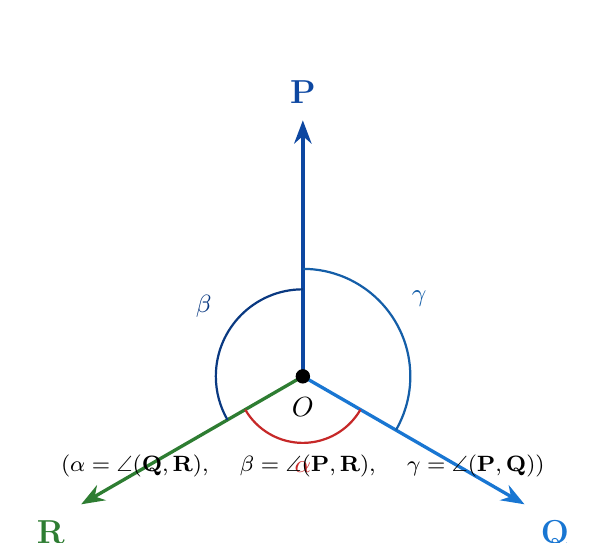
\begin{tikzpicture}[scale=1.3, >=Stealth]
    \coordinate (O) at (0,0);
    \coordinate (P) at (90:2.5);
    \coordinate (Q) at (-30:2.5);
    \coordinate (R) at (210:2.5);

    \draw[very thick, ->, color=primary] (O) -- (P) node[above=2pt, font=\large\bfseries] {$\mathbf{P}$};
    \draw[very thick, ->, color=secondary] (O) -- (Q) node[below right=2pt, font=\large\bfseries] {$\mathbf{Q}$};
    \draw[very thick, ->, color=proofcolor] (O) -- (R) node[below left=2pt, font=\large\bfseries] {$\mathbf{R}$};

    \fill (O) circle (2pt) node[below=4pt] {$O$};

    \draw[thick, color=examcolor] (-30:0.65) arc (-30:-150:0.65) node[midway, below=3pt, font=\small\bfseries] {$\alpha$};
    \draw[thick, color=primary!80!black] (90:0.85) arc (90:210:0.85) node[midway, above left=2pt, font=\small\bfseries] {$\beta$};
    \draw[thick, color=secondary!80!black] (90:1.05) arc (90:-30:1.05) node[midway, above right=2pt, font=\small\bfseries] {$\gamma$};
    
    \node[below=25pt] at (O) {\footnotesize ($\alpha = \angle(\mathbf{Q},\mathbf{R})$, \quad $\beta = \angle(\mathbf{P},\mathbf{R})$, \quad $\gamma = \angle(\mathbf{P},\mathbf{Q})$)};
\end{tikzpicture}
\end{center}

\subsection{Moments and Couples}

\begin{definitionbox}{Moment of Force About a Point}
The moment of a force $\mathbf{F}$ acting at a point with position vector $\mathbf{r}$ relative to moment center $O$ is defined as:
\begin{equation}
\mathbf{M}_O = \mathbf{r} \times \mathbf{F}
\end{equation}
Scalar magnitude of moment:
\begin{equation}
M = F \cdot p
\end{equation}
where $p$ is the perpendicular distance from $O$ to the line of action of force $\mathbf{F}$.
\end{definitionbox}

\begin{center}
\begin{tikzpicture}[scale=1.2, >=Stealth]
    \coordinate (O) at (0,0);
    \coordinate (P) at (2.5,0);
    \coordinate (F1) at (2.5,2.2);

    \draw[thick, dashed, color=gray] (-0.5,2.2) -- (5.5,2.2) node[right] {Line of action of $\mathbf{F}$};
    \draw[very thick, ->, color=primary] (P) -- (F1) node[midway, left] {$\mathbf{F}$};
    \draw[thick, color=examcolor] (O) -- (0,2.2) node[midway, left] {$p$};
    \fill (O) circle (2pt) node[below left] {$O$};
    \fill (P) circle (2pt) node[below] {$P$};
    \draw (0.3,0) arc (0:90:0.3);
\end{tikzpicture}
\end{center}

\begin{definitionbox}{Moment of Force About a Line}
Let $\mathbf{F}$ be a force acting at a point and let $OZ$ be any line in space. Let $\theta$ be the angle between $\mathbf{F}$ and line $OZ$.
Resolving $\mathbf{F}$ into:
1. $F \cos\theta$ parallel to line $OZ$
2. $F \sin\theta$ perpendicular to line $OZ$

The moment of force $\mathbf{F}$ about line $OZ$ is defined as the scalar moment of component $F \sin\theta$ about the point of intersection of line $OZ$ with a plane perpendicular to $OZ$:
\begin{equation}
M_{OZ} = (\mathbf{r} \times \mathbf{F}) \cdot \hat{\mathbf{k}}
\end{equation}
\end{definitionbox}

\begin{theorembox}{Varignon's Theorem of Moments}
The algebraic sum of the moments of any two coplanar forces about any point in their plane is equal to the moment of their resultant about that same point:
\begin{equation}
\mathbf{M}_O(\mathbf{R}) = \mathbf{M}_O(\mathbf{P}) + \mathbf{M}_O(\mathbf{Q})
\end{equation}
\end{theorembox}

\begin{proofbox}{Vector Proof of Varignon's Theorem}
Let two forces $\mathbf{P}$ and $\mathbf{Q}$ act at point $A$ with position vector $\mathbf{r}$ relative to moment center $O$.
The resultant force $\mathbf{R}$ is $\mathbf{R} = \mathbf{P} + \mathbf{Q}$.
Taking the vector cross product with $\mathbf{r}$ from the left:
\[
\mathbf{r} \times \mathbf{R} = \mathbf{r} \times (\mathbf{P} + \mathbf{Q}) = (\mathbf{r} \times \mathbf{P}) + (\mathbf{r} \times \mathbf{Q})
\]
This proves that the vector moment of the resultant equals the sum of the vector moments of the individual forces.
\end{proofbox}

\begin{theorembox}{Theory of Couples}
A **couple** consists of two equal, opposite, and non-collinear parallel forces $(P, -P)$.
1. The vector sum of forces in a couple is zero ($\sum \mathbf{F} = \mathbf{0}$). A couple produces pure rotation.
2. The moment of a couple $G = P \cdot d$ (where $d$ is arm of couple) is **constant** and independent of the base point.
3. The resultant of any number of coplanar couples of moments $G_1, G_2, \dots, G_n$ is a single couple of moment $G = \sum_{i=1}^n G_i$.
\end{theorembox}

\subsection{Reduction of General Coplanar System of Forces}

\begin{theorembox}{Reduction Theorem for Coplanar Forces}
A system of coplanar forces $\mathbf{P}_1, \mathbf{P}_2, \dots, \mathbf{P}_n$ acting at points $(x_1, y_1), (x_2, y_2), \dots, (x_n, y_n)$ on a rigid body can be reduced to a single resultant force $(X, Y)$ acting at an arbitrary origin $O$, together with a single couple of moment $G$ about $O$:
\begin{align}
X &= \sum_{i=1}^n X_i, \qquad Y = \sum_{i=1}^n Y_i \\
G &= \sum_{i=1}^n (x_i Y_i - y_i X_i)
\end{align}
where $(X_i, Y_i)$ are the components of force $\mathbf{P}_i$.
Resultant Force Magnitude: $R = \sqrt{X^2 + Y^2}$ and direction $\tan\theta = Y/X$.
\end{theorembox}

\begin{proofbox}{Proof of Reduction Theorem}
Let force $\mathbf{P}_i$ act at point $A_i(x_i, y_i)$ with components $(X_i, Y_i)$.
Transferring component $X_i$ to origin $O(0,0)$ introduces:
1. Equal force $X_i$ at $O$
2. Couple of moment $-y_i X_i$

Transferring component $Y_i$ to origin $O(0,0)$ introduces:
1. Equal force $Y_i$ at $O$
2. Couple of moment $+x_i Y_i$

Summing over all $n$ forces:
- Total force along $X$-axis at $O$: $X = \sum X_i$
- Total force along $Y$-axis at $O$: $Y = \sum Y_i$
- Total couple moment about $O$: $G = \sum (x_i Y_i - y_i X_i)$
\end{proofbox}

\begin{theorembox}{Line of Action of Resultant Force}
If $R \neq 0$, the equation of the line of action of the resultant force $R$ relative to origin $O$ is:
\begin{equation}
xY - yX = G
\end{equation}
\end{theorembox}

\begin{proofbox}{Proof of Line of Action Equation}
Let the base point be shifted from origin $O(0,0)$ to a point $O'(\xi, \eta)$.
The force components remain $(X, Y)$, but the new couple moment about $O'$ becomes:
\[
G' = G - \xi Y + \eta X
\]
For $O'(\xi, \eta)$ to lie on the line of action of resultant force $R$, the couple moment $G'$ must vanish ($G' = 0$):
\[
G - \xi Y + \eta X = 0 \implies \xi Y - \eta X = G
\]
Replacing coordinates $(\xi, \eta)$ with standard rectangular coordinates $(x, y)$ gives:
\[
xY - yX = G
\]
\end{proofbox}

\subsection{Laws of Friction and Equilibrium on Rough Surfaces}

\begin{definitionbox}{Friction and Limiting Friction}
1. \textbf{Friction}: The tangential force exerted by a rough surface on a body resting on it, opposing relative motion.
2. \textbf{Laws of Limiting Friction}:
   - Limiting friction $F_{\max} = \mu N$, where $\mu$ is the coefficient of static friction and $N$ is normal reaction.
   - Angle of Friction $\lambda = \tan^{-1}\mu$.
   - Cone of Friction: Right circular cone of semi-vertical angle $\lambda = \tan^{-1}\mu$ with axis along normal reaction $N$.
\end{definitionbox}

\begin{examplebox}{Equilibrium of Body on Rough Inclined Plane}
A heavy body of weight $W$ rests on a rough inclined plane of inclination $\alpha$ to horizontal. Find the minimum horizontal force $P$ required to prevent the body from sliding down the plane.
\end{examplebox}

\begin{proofbox}{Solution}
Let $\lambda$ be the angle of friction ($\mu = \tan\lambda$).
When the body is on the verge of sliding down, friction $F = \mu N$ acts up the plane.
Resolving forces along and perpendicular to the inclined plane:
\begin{align}
P \cos\alpha + F &= W \sin\alpha \implies F = W \sin\alpha - P \cos\alpha \\
N &= W \cos\alpha + P \sin\alpha
\end{align}
Setting limiting friction $F = \mu N = N \tan\lambda$:
\[
W \sin\alpha - P \cos\alpha = (W \cos\alpha + P \sin\alpha) \frac{\sin\lambda}{\cos\lambda}
\]
Cross-multiplying by $\cos\lambda$:
\[
W (\sin\alpha \cos\lambda - \cos\alpha \sin\lambda) = P (\cos\alpha \cos\lambda + \sin\alpha \sin\lambda)
\]
\[
W \sin(\alpha - \lambda) = P \cos(\alpha - \lambda) \implies P = W \tan(\alpha - \lambda)
\]
\end{proofbox}

\subsection{Solved Standard Exam Problems from Part I}

\begin{examplebox}{Forces Along Sides of Triangle $AB, BC, CA$}
Forces equal to $3P, 7P, 5P$ act along the sides $AB, BC, CA$ of an equilateral triangle $ABC$ of side $a$, taken in order. Find the magnitude, direction, and line of action of the resultant force.
\end{examplebox}

\begin{proofbox}{Solution}
Let side $AB$ lie along the $X$-axis with $A$ at origin $(0,0)$.
Side angles with $X$-axis: $0^\circ$ for $AB$, $120^\circ$ for $BC$, $240^\circ$ for $CA$.

1. **Horizontal Component $X$**:
\[
X = 3P \cos 0^\circ + 7P \cos 120^\circ + 5P \cos 240^\circ = 3P + 7P\left(-\frac{1}{2}\right) + 5P\left(-\frac{1}{2}\right) = -3P
\]

2. **Vertical Component $Y$**:
\[
Y = 3P \sin 0^\circ + 7P \sin 120^\circ + 5P \sin 240^\circ = 0 + 7P\left(\frac{\sqrt{3}}{2}\right) + 5P\left(-\frac{\sqrt{3}}{2}\right) = \sqrt{3}P
\]

3. **Resultant Magnitude and Direction**:
\[
R = \sqrt{X^2 + Y^2} = \sqrt{(-3P)^2 + (\sqrt{3}P)^2} = \sqrt{12P^2} = 2\sqrt{3}P
\]
\[
\tan\theta = \frac{Y}{X} = \frac{\sqrt{3}P}{-3P} = -\frac{1}{\sqrt{3}} \implies \theta = 150^\circ
\]

4. **Resultant Moment $G_A$ about $A$**:
Taking moments about vertex $A(0,0)$:
Forces $3P$ and $5P$ pass through $A \implies \text{moments } = 0$.
Perpendicular distance from $A$ to line $BC$ is $p = a\sin 60^\circ = \frac{\sqrt{3}}{2}a$.
\[
G_A = 7P \cdot \left(\frac{\sqrt{3}}{2}a\right) = \frac{7\sqrt{3}}{2}Pa
\]
Line of action equation $xY - yX = G_A$:
\[
x(\sqrt{3}P) - y(-3P) = \frac{7\sqrt{3}}{2}Pa \implies \sqrt{3}x + 3y = \frac{7\sqrt{3}}{2}a \implies 2x + 2\sqrt{3}y = 7a
\]
\end{proofbox}

\begin{examplebox}{Forces Along Sides of Regular Hexagon}
$ABCDEF$ is a regular hexagon of side $a$. Forces $P, 2P, 3P, 4P, 5P, 6P$ act along sides $AB, BC, CD, DE, EF, FA$ respectively. Find the magnitude, direction, and line of action of the resultant.
\end{examplebox}

\begin{proofbox}{Solution}
Let side $AB$ lie along $X$-axis with $A$ at origin $(0,0)$.
Angles of sides with $X$-axis: $0^\circ, 60^\circ, 120^\circ, 180^\circ, 240^\circ, 300^\circ$.

1. **Resolution**:
\[
X = P\cos 0^\circ + 2P\cos 60^\circ + 3P\cos 120^\circ + 4P\cos 180^\circ + 5P\cos 240^\circ + 6P\cos 300^\circ = -3P
\]
\[
Y = P\sin 0^\circ + 2P\sin 60^\circ + 3P\sin 120^\circ + 4P\sin 180^\circ + 5P\sin 240^\circ + 6P\sin 300^\circ = -3\sqrt{3}P
\]
\[
R = \sqrt{(-3P)^2 + (-3\sqrt{3}P)^2} = 6P, \qquad \tan\theta = \sqrt{3} \implies \theta = 240^\circ
\]

2. **Moment about Center $O$**:
Perpendicular distance to any side is $p = \frac{\sqrt{3}}{2}a$.
\[
G_O = (P + 2P + 3P + 4P + 5P + 6P) \frac{\sqrt{3}}{2}a = 21P \cdot \frac{\sqrt{3}}{2}a = \frac{21\sqrt{3}}{2}Pa
\]
\end{proofbox}

% =========================================================================
\section{Part II: Principle of Virtual Work \& Stability}
% =========================================================================

\subsection{Principle of Virtual Work}

\begin{theorembox}{Principle of Virtual Work}
A system of coplanar forces acting on a rigid body or interconnected system with ideal workless constraints is in **static equilibrium** if and only if the total virtual work done by all external forces in any arbitrary virtual displacement consistent with constraints vanishes:
\begin{equation}
\sum \delta W = 0
\end{equation}
\end{theorembox}

\begin{proofbox}{Virtual Work for Common Constraint Forces}
1. **Extensible / Inextensible String**: $\delta W = -T \delta s$. For inextensible string ($\delta s = 0$), $\delta W = 0$.
2. **Light Rigid Rod**: $\delta W = -R \delta l$. For rigid rod ($\delta l = 0$), $\delta W = 0$.
3. **Smooth Surface Reaction**: Normal reaction $N \perp \delta \mathbf{r} \implies \delta W = N \cdot 0 = 0$.
4. **Fixed Smooth Hinge**: Point of application does not move $\implies \delta W = 0$.
5. **Gravity Force**: $\delta W = -W \delta y_{cg}$.
\end{proofbox}

\subsection{Solved Examples on Jointed Frameworks}

\begin{examplebox}{Four Jointed Uniform Rods Forming Rhombus}
Four equal uniform rods, each of weight $w$ and length $a$, are freely jointed to form a rhombus $ABCD$. The framework is suspended vertically from vertex $A$. A weight $W$ is attached at the lowest vertex $C$, and the framework is kept in shape by a light inextensible string joining $B$ and $D$. If $\angle DAB = 2\theta$, find the tension $T$ in string $BD$.
\end{examplebox}

\begin{proofbox}{Solution using Virtual Work}
Let $A$ be the fixed origin $(0,0)$ with $Y$-axis vertically downwards.
1. **Coordinates**:
   - Depth of vertex $C$: $y_C = 2a\cos\theta$.
   - Depth of center of gravity of 4 rods: $y_{cg} = a\cos\theta$. Total weight of 4 rods = $4w$.
   - Length of diagonal $BD$: $x = 2a\sin\theta$.

2. **Virtual Work Equation**:
   Active forces are weight $W$ at $C$, weight $4w$ at center of gravity, and tension $T$ along $BD$:
   \begin{equation}
   \delta W = W \delta y_C + 4w \delta y_{cg} - T \delta x = 0
   \end{equation}

3. **Differentiating Coordinates**:
   - $\delta y_C = -2a\sin\theta \, \delta\theta$
   - $\delta y_{cg} = -a\sin\theta \, \delta\theta$
   - $\delta x = 2a\cos\theta \, \delta\theta$

4. **Substitution**:
   \[
   W(-2a\sin\theta \, \delta\theta) + 4w(-a\sin\theta \, \delta\theta) - T(2a\cos\theta \, \delta\theta) = 0
   \]
   Dividing by $-2a\delta\theta$:
   \[
   W\sin\theta + 2w\sin\theta + T\cos\theta = 0 \implies T = (2w + W) \tan\theta
   \]
\end{proofbox}

\begin{examplebox}{Six Jointed Equal Rods Forming Regular Hexagon}
Six equal rods $AB, BC, CD, DE, EF, FA$, each of weight $w$, are jointed together to form a regular hexagon $ABCDEF$. The framework is suspended vertically from vertex $A$, and a weight $W$ is attached at lowest vertex $D$. A light horizontal string joins the midpoints of $AB$ and $AF$. Find the tension $T$ in the string using Virtual Work.
\end{examplebox}

\begin{proofbox}{Solution}
Let $\theta$ be the angle each upper rod makes with the vertical diagonal $AD$. For a regular hexagon, $\theta = 30^\circ$.
1. **Coordinates**:
   - Depth of lowest vertex $D$: $y_D = 4a\cos\theta$.
   - Depth of center of gravity of 6 rods: $y_{cg} = 2a\cos\theta$. Total weight = $6w$.
   - Distance between midpoints of $AB$ and $AF$: $x = a\sin\theta$.

2. **Virtual Work Equation**:
   \[
   \delta W = W \delta y_D + 6w \delta y_{cg} - T \delta x = 0
   \]
   \[
   W(-4a\sin\theta \, \delta\theta) + 6w(-2a\sin\theta \, \delta\theta) - T(a\cos\theta \, \delta\theta) = 0
   \]
   Dividing by $a\delta\theta$:
   \[
   T\cos\theta = (4W + 12w)\sin\theta \implies T = (4W + 12w)\tan\theta
   \]
   For $\theta = 30^\circ$, $\tan 30^\circ = \frac{1}{\sqrt{3}}$:
   \begin{equation}
   T = \frac{4W + 12w}{\sqrt{3}} = \frac{4}{\sqrt{3}}(W + 3w)
   \end{equation}
\end{proofbox}

\subsection{Stability of Equilibrium and Potential Energy Criteria}

\begin{theorembox}{Potential Energy Criterion for Stability}
For conservative systems with potential energy $V(\theta)$:
- **Equilibrium**: $\frac{dV}{d\theta} = 0$
- **Stable Equilibrium**: $\frac{d^2V}{d\theta^2} > 0$ (Local Minimum of $V$)
- **Unstable Equilibrium**: $\frac{d^2V}{d\theta^2} < 0$ (Local Maximum of $V$)
\end{theorembox}

\begin{theorembox}{Stability Criterion for Curved Surfaces}
If a body of radius of curvature $r$ rests on top of a fixed convex surface of radius of curvature $R$ with center of gravity at height $h$ above contact point:
- **Stable**: $\frac{1}{h} > \frac{1}{r} + \frac{1}{R}$
- **Unstable**: $\frac{1}{h} < \frac{1}{r} + \frac{1}{R}$
\end{theorembox}

% =========================================================================
\section{Part III: Common Catenary \& Flexible Strings}
% =========================================================================

\subsection{Intrinsic and Cartesian Equations of Common Catenary}

\begin{definitionbox}{Common Catenary}
A \textbf{common catenary} is the curve formed by a uniform, flexible, inextensible string hanging freely under gravity between two fixed points.
\end{definitionbox}

\begin{center}
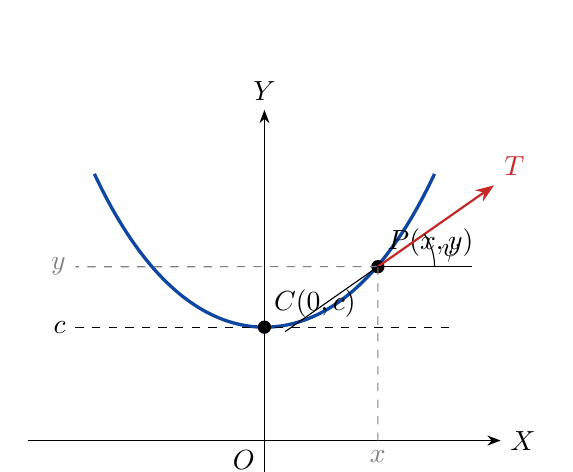
\begin{tikzpicture}[scale=1.2, >=Stealth]
    \draw[->] (-0.5,0) -- (4.5,0) node[right] {$X$};
    \draw[->] (2,-0.5) -- (2,3.5) node[above] {$Y$};
    \node[below left] at (2,0) {$O$};

    \draw[very thick, color=primary, domain=-1.8:1.8, samples=100] plot ({\x+2}, {1.2*cosh(\x/1.2)});

    \fill (2,1.2) circle (2pt) node[above right] {$C(0,c)$};
    \draw[dashed] (0,1.2) -- (4,1.2);
    \node[left] at (0,1.2) {$c$};

    \coordinate (P) at (3.2, 1.84);
    \fill (P) circle (2pt) node[above right] {$P(x,y)$};

    \draw[thick, ->, color=examcolor] (P) -- +(35:1.5) node[above right] {$T$};
    \draw[dashed, color=gray] (P) -- (3.2,0) node[below] {$x$};
    \draw[dashed, color=gray] (P) -- (0,1.84) node[left] {$y$};

    \draw (P) -- +(-145:1.2);
    \draw (P) +(0:0) -- +(0:1.0);
    \draw (P) +(0.6,0) arc (0:35:0.6) node[midway, right] {$\psi$};
\end{tikzpicture}
\end{center}

\begin{proofbox}{Derivation of Intrinsic Equation $s = c \tan\psi$}
Consider an arc $CP$ of length $s$ measured from lowest point $C(0,c)$ to point $P(x,y)$.
Let $w$ be the weight per unit length of string.
Three forces keep arc $CP$ in equilibrium:
1. Horizontal tension $T_0$ at lowest point $C$.
2. Tension $T$ at $P$ acting along tangent at angle $\psi$ to horizontal.
3. Weight of arc $CP$, $W = w s$, acting vertically downwards.

Resolving forces:
\begin{align}
T \cos\psi &= T_0 \label{eq:fullcat1_d} \\
T \sin\psi &= w s \label{eq:fullcat2_d}
\end{align}
Dividing (\ref{eq:fullcat2_d}) by (\ref{eq:fullcat1_d}):
\[
\tan\psi = \frac{ws}{T_0} \implies s = \left(\frac{T_0}{w}\right) \tan\psi = c \tan\psi
\]
where parameter $c = \frac{T_0}{w}$.
\end{proofbox}

\begin{proofbox}{Derivation of Cartesian Equation $y = c \cosh(x/c)$}
From calculus, $\frac{dy}{dx} = \tan\psi$ and $\frac{ds}{dx} = \sec\psi$.
Differentiating $s = c \tan\psi$ with respect to $x$:
\[
\frac{ds}{dx} = c \sec^2\psi \frac{d\psi}{dx} \implies \sec\psi = c \sec^2\psi \frac{d\psi}{dx} \implies dx = c \sec\psi \, d\psi
\]
Integrating $dx = c \sec\psi \, d\psi$:
\[
x = c \ln(\sec\psi + \tan\psi) \implies \sec\psi + \tan\psi = e^{x/c}
\]
Since $\sec\psi - \tan\psi = e^{-x/c}$, adding gives $2\sec\psi = e^{x/c} + e^{-x/c} \implies \sec\psi = \cosh(x/c)$.
Integrating $\frac{dy}{dx} = \tan\psi = \sinh(x/c)$ with $y(0) = c$:
\begin{equation}
y = c \cosh\left(\frac{x}{c}\right)
\end{equation}
\end{proofbox}

\begin{importantbox}{Master Relations for Common Catenary}
\begin{align}
y^2 &= c^2 + s^2 \\
T &= w y \\
T_0 &= w c \\
x &= c \ln(\sec\psi + \tan\psi) = c \sinh^{-1}\left(\frac{s}{c}\right)
\end{align}
\end{importantbox}

\subsection{Solved Examples on Catenary}

\begin{examplebox}{Tension at Any Point of Catenary}
Prove that the tension $T$ at any point $P(x,y)$ of a common catenary is equal to the weight of a length of the string equal to the height of $P$ above the directrix ($T = wy$).
\end{examplebox}

\begin{proofbox}{Proof}
Squaring and adding equations (\ref{eq:fullcat1_d}) and (\ref{eq:fullcat2_d}):
\[
T^2 (\cos^2\psi + \sin^2\psi) = T_0^2 + w^2 s^2 = w^2 c^2 + w^2 s^2 = w^2 (c^2 + s^2)
\]
Using the master relation $c^2 + s^2 = y^2$:
\[
T^2 = w^2 y^2 \implies T = w y
\]
This completes the proof.
\end{proofbox}

\begin{examplebox}{Length of String Given Span and Sag}
A uniform string of length $l$ hangs between two points in the same horizontal line. If the span is $2b$ and sag is $d$, show that:
\begin{equation}
y_A = c + d, \qquad (c+d)^2 = c^2 + \left(\frac{l}{2}\right)^2 \implies c = \frac{l^2 - 4d^2}{8d}
\end{equation}
\end{examplebox}

\begin{proofbox}{Solution}
At the support point $A(b, y_A)$, half-length of string is $s = l/2$.
Height of $A$ above directrix: $y_A = c + d$.
Using $y^2 = c^2 + s^2$:
\[
(c + d)^2 = c^2 + \left(\frac{l}{2}\right)^2 \implies c^2 + 2cd + d^2 = c^2 + \frac{l^2}{4}
\]
\[
2cd + d^2 = \frac{l^2}{4} \implies 2cd = \frac{l^2 - 4d^2}{4} \implies c = \frac{l^2 - 4d^2}{8d}
\]
\end{proofbox}

% =========================================================================
\section{Part IV: Kinematics, Rectilinear Motion \& Simple Harmonic Motion}
% =========================================================================

\subsection{Kinematics in 2D Systems}

\begin{theorembox}{Expressions for Velocity and Acceleration}
1. **Cartesian Coordinates $(x, y)$**:
   - Velocity: $\mathbf{v} = \dot{x}\hat{\mathbf{i}} + \dot{y}\hat{\mathbf{j}}$, magnitude $v = \sqrt{\dot{x}^2 + \dot{y}^2}$
   - Acceleration: $\mathbf{a} = \ddot{x}\hat{\mathbf{i}} + \ddot{y}\hat{\mathbf{j}}$, magnitude $a = \sqrt{\ddot{x}^2 + \ddot{y}^2}$

2. **Polar Coordinates $(r, \theta)$**:
   - Radial velocity: $v_r = \dot{r}$
   - Transverse velocity: $v_\theta = r\dot{\theta}$
   - Radial acceleration: $a_r = \ddot{r} - r\dot{\theta}^2$
   - Transverse acceleration: $a_\theta = \frac{1}{r}\frac{d}{dt}(r^2\dot{\theta}) = r\ddot{\theta} + 2\dot{r}\dot{\theta}$

3. **Intrinsic Coordinates $(s, \psi)$**:
   - Tangential velocity: $v_t = \dot{s}$
   - Normal velocity: $v_n = 0$
   - Tangential acceleration: $a_t = \frac{dv}{dt} = v\frac{dv}{ds} = \ddot{s}$
   - Normal acceleration: $a_n = \frac{v^2}{\rho}$ (where $\rho = \frac{ds}{d\psi}$)
\end{theorembox}

\subsection{Simple Harmonic Motion (SHM)}

\begin{definitionbox}{Simple Harmonic Motion}
A particle moves in a straight line with **Simple Harmonic Motion** if its acceleration is always directed towards a fixed point $O$ on the line and is directly proportional to its displacement $x$ from $O$:
\begin{equation}
\ddot{x} = -\mu x \quad (\mu > 0)
\end{equation}
\end{definitionbox}

\begin{proofbox}{Derivation of Velocity and Position in SHM}
Writing $\ddot{x} = v \frac{dv}{dx} = -\mu x$:
\[
v \, dv = -\mu x \, dx \implies \frac{v^2}{2} = -\mu \frac{x^2}{2} + C_1
\]
If particle comes to rest at maximum displacement $x = a$ (Amplitude):
\[
0 = -\frac{1}{2}\mu a^2 + C_1 \implies C_1 = \frac{1}{2}\mu a^2
\]
\begin{equation}
v^2 = \mu (a^2 - x^2) \implies v = \pm \sqrt{\mu} \sqrt{a^2 - x^2}
\end{equation}

For motion starting from rest at $x = a$:
\[
\frac{dx}{dt} = -\sqrt{\mu} \sqrt{a^2 - x^2} \implies \frac{dx}{\sqrt{a^2 - x^2}} = -\sqrt{\mu} \, dt
\]
Integrating with $x(0) = a$:
\begin{equation}
\cos^{-1}\left(\frac{x}{a}\right) = \sqrt{\mu} t \implies x(t) = a \cos(\sqrt{\mu} t)
\end{equation}

**Periodic Time $T$**:
\begin{equation}
T = \frac{2\pi}{\sqrt{\mu}}
\end{equation}
\end{proofbox}

\begin{center}
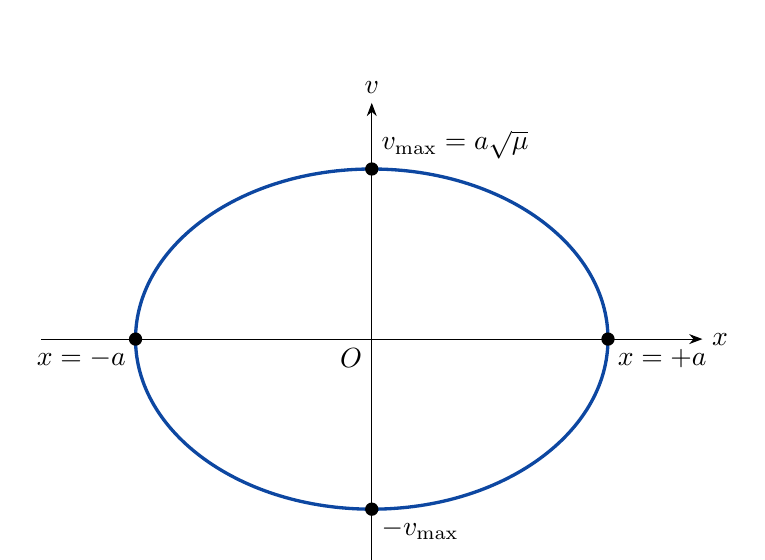
\begin{tikzpicture}[scale=1.2, >=Stealth]
    \draw[->] (-3.5,0) -- (3.5,0) node[right] {$x$};
    \draw[->] (0,-2.5) -- (0,2.5) node[above] {$v$};

    \draw[very thick, color=primary] (0,0) ellipse (2.5 and 1.8);

    \node[below left] at (0,0) {$O$};
    \fill (2.5,0) circle (2pt) node[below right] {$x = +a$};
    \fill (-2.5,0) circle (2pt) node[below left] {$x = -a$};
    \fill (0,1.8) circle (2pt) node[above right] {$v_{\max} = a\sqrt{\mu}$};
    \fill (0,-1.8) circle (2pt) node[below right] {$-v_{\max}$};
\end{tikzpicture}
\end{center}

\begin{examplebox}{Velocities at Two Positions in SHM}
A point executing SHM has velocities $v_1$ and $v_2$ at distances $x_1$ and $x_2$ from the center of force. Find the amplitude $a$ and period $T$ of the motion.
\end{examplebox}

\begin{proofbox}{Solution}
Using $v^2 = \mu(a^2 - x^2)$ at the two given positions:
\begin{align}
v_1^2 &= \mu(a^2 - x_1^2) \label{eq:shm1_d} \\
v_2^2 &= \mu(a^2 - x_2^2) \label{eq:shm2_d}
\end{align}
Subtracting (\ref{eq:shm2_d}) from (\ref{eq:shm1_d}):
\[
v_1^2 - v_2^2 = \mu (x_2^2 - x_1^2) \implies \mu = \frac{v_1^2 - v_2^2}{x_2^2 - x_1^2}
\]
Periodic time $T$:
\begin{equation}
T = \frac{2\pi}{\sqrt{\mu}} = 2\pi \sqrt{\frac{x_2^2 - x_1^2}{v_1^2 - v_2^2}}
\end{equation}
To find amplitude $a$, multiply (\ref{eq:shm1_d}) by $x_2^2$ and (\ref{eq:shm2_d}) by $x_1^2$ and subtract:
\[
v_1^2 x_2^2 - v_2^2 x_1^2 = \mu a^2 (x_2^2 - x_1^2) = (v_1^2 - v_2^2) a^2 \implies a = \sqrt{\frac{v_1^2 x_2^2 - v_2^2 x_1^2}{v_1^2 - v_2^2}}
\]
\end{proofbox}

\subsection{Motion in Resisting Medium}

\begin{theorembox}{Motion Under Resistance Proportional to Velocity}
If a body of mass $m$ falls vertically under gravity in a medium with resistance $m k v$:
Equation of motion: $\ddot{x} = g - k v$.
Setting $\ddot{x} = 0$ gives the **Terminal Velocity $V$**:
\begin{equation}
V = \frac{g}{k}
\end{equation}
\end{theorembox}

% =========================================================================
\section{Part V: Central Orbits \& Kepler's Laws}
% =========================================================================

\subsection{Differential Equations of Central Orbits}

\begin{theorembox}{Differential Equation in $u - \theta$ Form}
Let a particle move under a central attractive force $P(r)$ per unit mass towards pole $O$.
Since transverse acceleration $a_\theta = 0 \implies r^2\dot{\theta} = h = \text{constant}$ (Areal velocity $\frac{1}{2}h = \text{constant}$).

Substituting $u = 1/r$ into radial equation $\ddot{r} - r\dot{\theta}^2 = -P$ yields the standard differential equation:
\begin{equation}
\frac{d^2 u}{d\theta^2} + u = \frac{P}{h^2 u^2}
\end{equation}
\end{theorembox}

\begin{theorembox}{Pedal Equation ($p-r$) of Central Orbit}
In pedal coordinates $(p, r)$ where $p = r\sin\phi = r^2 \frac{d\theta}{ds}$:
\begin{equation}
\frac{h^2}{p^3} \frac{dp}{dr} = P
\end{equation}
\end{theorembox}

\subsection{Kepler's Laws of Planetary Motion}

\begin{theorembox}{Kepler's Laws}
1. **First Law (Law of Orbits)**: Every planet moves in an ellipse with the Sun at one focus.
2. **Second Law (Law of Areas)**: Radius vector from Sun sweeps equal areas in equal times ($\frac{dA}{dt} = \frac{1}{2}h = \text{constant}$).
3. **Third Law (Law of Periods)**: Period $T$ satisfies:
\begin{equation}
T^2 = \frac{4\pi^2}{\mu} a^3 \implies T^2 \propto a^3
\end{equation}
\end{theorembox}

\subsection{Solved Examples on Central Force Laws}

\begin{examplebox}{Law of Force for Central Elliptic Orbit}
Find the law of force towards the focus for a particle describing an ellipse $\frac{l}{r} = 1 + e\cos\theta$.
\end{examplebox}

\begin{proofbox}{Solution}
Writing $u = \frac{1}{r} = \frac{1}{l}(1 + e\cos\theta)$.
Differentiating with respect to $\theta$:
\[
\frac{du}{d\theta} = -\frac{e}{l}\sin\theta \implies \frac{d^2 u}{d\theta^2} = -\frac{e}{l}\cos\theta
\]
Substituting into differential equation $\frac{d^2 u}{d\theta^2} + u = \frac{P}{h^2 u^2}$:
\[
-\frac{e}{l}\cos\theta + \frac{1}{l}(1 + e\cos\theta) = \frac{P}{h^2 u^2} \implies \frac{1}{l} = \frac{P}{h^2 u^2}
\]
Solving for central force $P$:
\begin{equation}
P = \frac{h^2}{l} u^2 = \frac{\mu}{r^2} \quad \text{where } \mu = \frac{h^2}{l}
\end{equation}
Thus the central force obeys the **Inverse Square Law**.
\end{proofbox}

\begin{examplebox}{Law of Force for Equiangular Spiral}
Find the law of force for a particle describing an equiangular spiral $r = a e^{\theta\cot\alpha}$ under a central force towards the pole.
\end{examplebox}

\begin{proofbox}{Solution}
Pedal equation of equiangular spiral is $p = r\sin\alpha$.
Differentiating with respect to $r$: $\frac{dp}{dr} = \sin\alpha$.
Substituting into pedal differential equation $\frac{h^2}{p^3}\frac{dp}{dr} = P$:
\[
P = \frac{h^2}{(r\sin\alpha)^3} \sin\alpha = \frac{h^2}{\sin^2\alpha} \cdot \frac{1}{r^3} = \frac{\mu}{r^3}
\]
Thus the force varies inversely as the **cube** of the distance.
\end{proofbox}

% =========================================================================
\section{Part VI: Constrained Motion on Curves}
% =========================================================================

\subsection{Motion on a Smooth Vertical Circle}

\begin{examplebox}{Complete Vertical Loop Condition}
A particle of mass $m$ is projected horizontally with velocity $u$ from the lowest point of a smooth vertical circle of radius $a$. Find the minimum velocity $u$ required for the particle to complete the full vertical circle.
\end{examplebox}

\begin{proofbox}{Solution}
Let $\theta$ be the angle of radius vector with lowest vertical.
By Conservation of Energy:
\[
\frac{1}{2}m v^2 + mga(1 - \cos\theta) = \frac{1}{2}m u^2 \implies v^2 = u^2 - 2ga(1 - \cos\theta)
\]
Normal reaction $N$:
\[
N - mg\cos\theta = \frac{m v^2}{a} \implies N = \frac{m}{a}\left[u^2 - 2ga + 3ga\cos\theta\right]
\]
At highest point $\theta = 180^\circ$ ($\cos 180^\circ = -1$):
\[
v_{\top}^2 = u^2 - 4ga, \qquad N_{\top} = \frac{m}{a}(u^2 - 5ga)
\]
To complete the loop without leaving the circle, $N_{\top} \ge 0$:
\[
u^2 - 5ga \ge 0 \implies u \ge \sqrt{5ga}
\]
\end{proofbox}

\subsection{Motion on a Smooth Cycloid}

\begin{theorembox}{Cycloidal Pendulum}
For a particle constrained to move under gravity along a smooth cycloid $s = 4a\sin\psi$:
Equation of motion: $\ddot{s} = -g\sin\psi = -\frac{g}{4a} s$.
This is exact **Simple Harmonic Motion** with periodic time:
\begin{equation}
T = 2\pi \sqrt{\frac{4a}{g}} = 4\pi \sqrt{\frac{a}{g}}
\end{equation}
Since period $T$ is independent of amplitude, motion on a cycloid is **isochronous**.
\end{theorembox}

% =========================================================================
\section{Part VII: Rotating Reference Frames \& Coriolis Force}
% =========================================================================

\subsection{Coriolis Acceleration and Coriolis Force}

\begin{theorembox}{Transformation to Rotating Frame}
If a frame of reference rotates with constant angular velocity $\boldsymbol{\omega}$ relative to an inertial frame, the relationship between time derivatives of vector $\mathbf{A}$ in fixed frame $(F)$ and rotating frame $(R)$ is:
\begin{equation}
\left(\frac{d\mathbf{A}}{dt}\right)_F = \left(\frac{d\mathbf{A}}{dt}\right)_R + \boldsymbol{\omega} \times \mathbf{A}
\end{equation}
Applying this transformation twice to position vector $\mathbf{r}$ yields the **Apparent Acceleration**:
\begin{equation}
\mathbf{a}_F = \mathbf{a}_R + 2(\boldsymbol{\omega} \times \mathbf{v}_R) + \boldsymbol{\omega} \times (\boldsymbol{\omega} \times \mathbf{r})
\end{equation}
Multiplying by mass $m$ gives Newton's Second Law in rotating frame:
\begin{equation}
m \mathbf{a}_R = \mathbf{F}_{\text{real}} - \underbrace{2m (\boldsymbol{\omega} \times \mathbf{v}_R)}_{\text{Coriolis Force}} - \underbrace{m \boldsymbol{\omega} \times (\boldsymbol{\omega} \times \mathbf{r})}_{\text{Centrifugal Force}}
\end{equation}
\end{theorembox}

% =========================================================================
\section{Master Formula Cheat Sheet (Exam Reference)}
% =========================================================================

\begin{importantbox}{Master Formula Reference Cheat Sheet}
\begin{enumerate}[leftmargin=1.5em]
    \item \textbf{Coplanar Resultant}:
    \[ R = \sqrt{R_x^2 + R_y^2}, \qquad \tan\theta = \frac{R_y}{R_x}, \qquad x Y - y X = G \]
    \item \textbf{Lami's Theorem}:
    \[ \frac{P}{\sin\alpha} = \frac{Q}{\sin\beta} = \frac{R}{\sin\gamma} \]
    \item \textbf{Limiting Friction \& Angle of Friction}:
    \[ F_{\max} = \mu N, \qquad \tan\lambda = \mu, \qquad P_{\min} = W\tan(\alpha-\lambda) \]
    \item \textbf{Principle of Virtual Work}:
    \[ \sum \delta W = 0 \quad (\text{Strings: } -T\delta s, \, \text{Rods: } -R\delta l, \, \text{Gravity: } -W\delta y_{cg}) \]
    \item \textbf{Equilibrium Stability}:
    \[ \frac{dV}{d\theta} = 0 \implies \text{Equilibrium}, \quad \frac{d^2V}{d\theta^2} > 0 \implies \text{Stable}, \quad \frac{1}{h} > \frac{1}{r} + \frac{1}{R} \]
    \item \textbf{Common Catenary}:
    \[ s = c\tan\psi, \quad y = c\cosh(x/c), \quad y^2 = c^2+s^2, \quad T = wy, \quad T_0 = wc \]
    \item \textbf{Kinematics \& SHM}:
    \[ v_r = \dot{r}, \; v_\theta = r\dot{\theta}, \; a_r = \ddot{r}-r\dot{\theta}^2, \; a_\theta = \frac{1}{r}\frac{d}{dt}(r^2\dot{\theta}) \]
    \[ \ddot{x} = -\mu x \implies v^2 = \mu(a^2-x^2), \quad T = \frac{2\pi}{\sqrt{\mu}}, \quad x(t) = a\cos(\sqrt{\mu}t) \]
    \item \textbf{Central Orbits \& Kepler}:
    \[ \frac{d^2u}{d\theta^2} + u = \frac{P}{h^2 u^2}, \qquad \frac{h^2}{p^3}\frac{dp}{dr} = P, \qquad T^2 = \frac{4\pi^2}{\mu}a^3 \]
    \item \textbf{Constrained Vertical Motion}:
    \[ v^2 = u^2 - 2ga(1-\cos\theta), \quad N = \frac{m}{a}[u^2 - 2ga + 3ga\cos\theta], \quad u_{\text{loop}} \ge \sqrt{5ga} \]
    \[ \text{Cycloid: } s = 4a\sin\psi \implies \ddot{s} = -\frac{g}{4a}s \implies T = 4\pi\sqrt{\frac{a}{g}} \]
    \item \textbf{Coriolis \& Centrifugal Forces}:
    \[ \mathbf{F}_{\text{Coriolis}} = -2m(\boldsymbol{\omega} \times \mathbf{v}_R), \qquad \mathbf{F}_{\text{centrifugal}} = -m\boldsymbol{\omega} \times (\boldsymbol{\omega} \times \mathbf{r}) \]
\end{enumerate}
\end{importantbox}

\end{document}
